\begin{figure}
\begin{center}
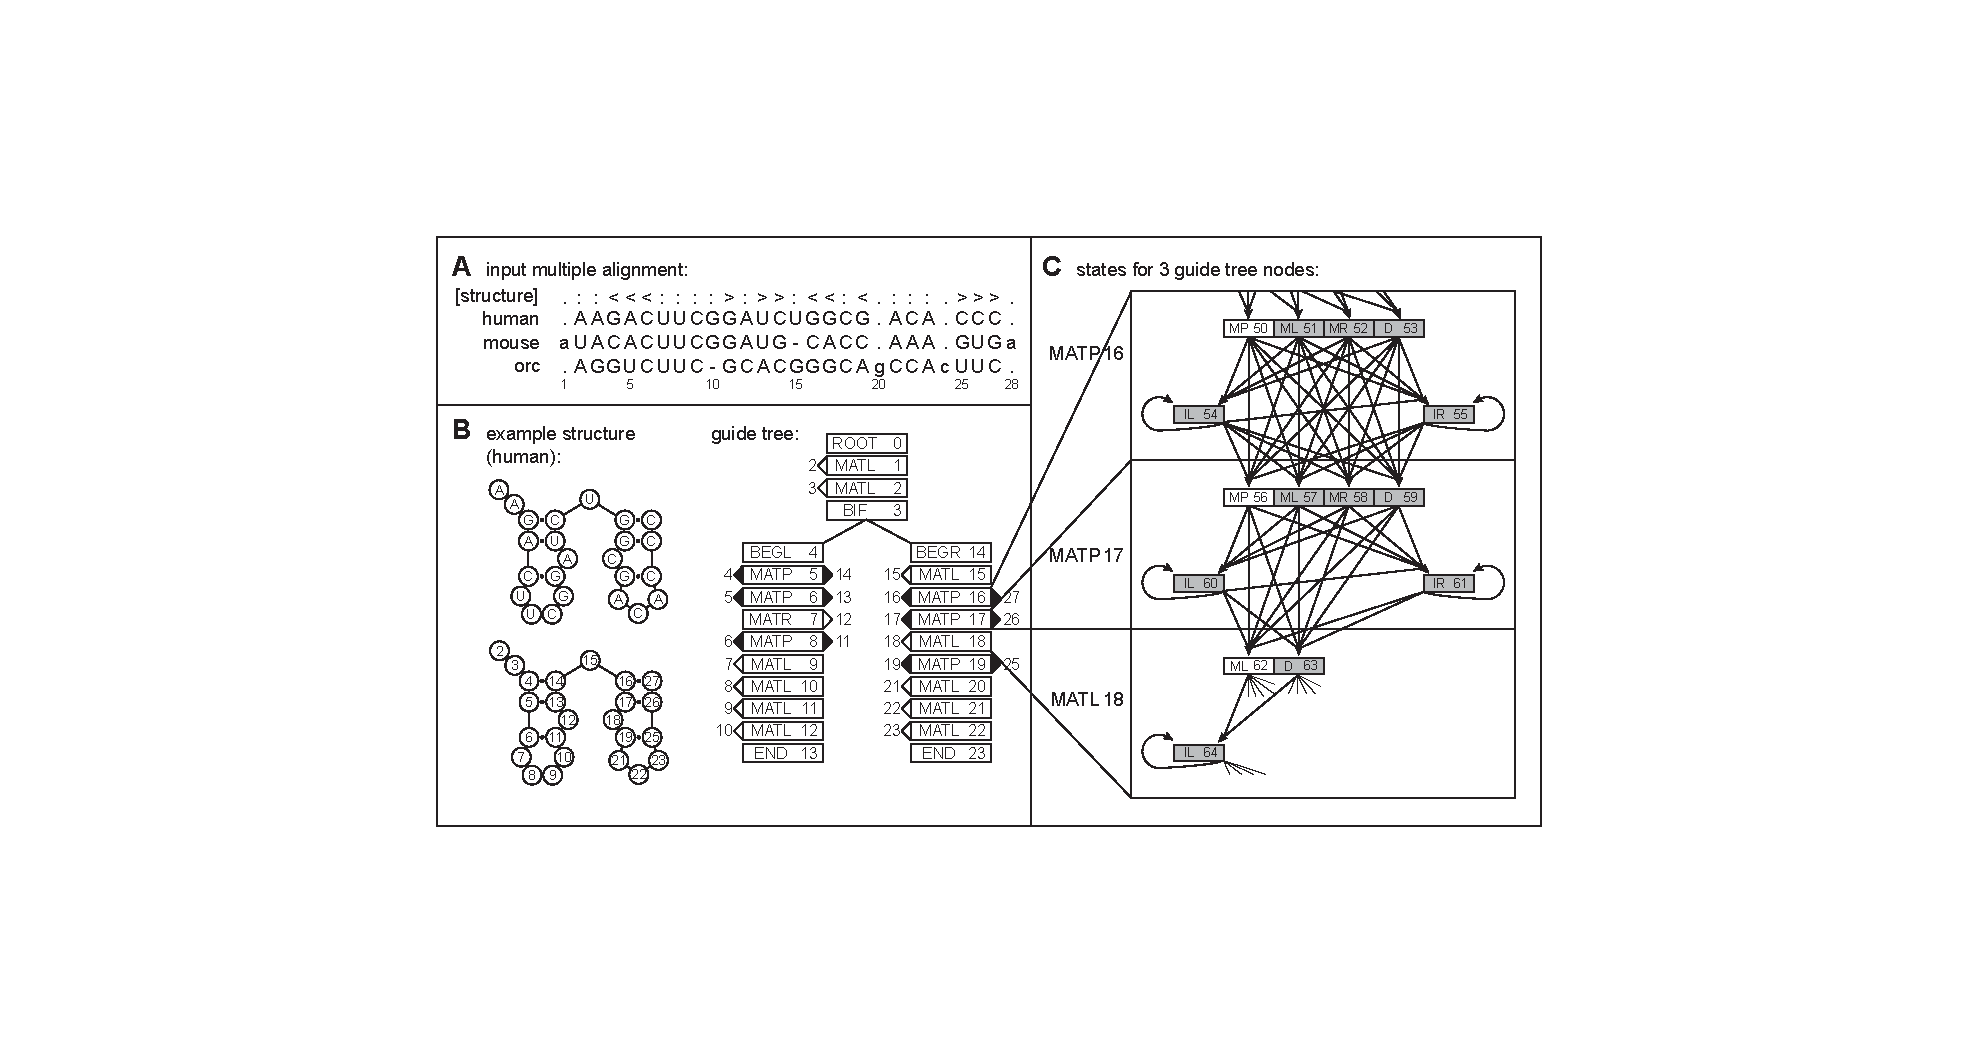
\includegraphics[width=6.4in]{figs/cmintro_bandcyk}
\caption{\textbf{An example RNA family and corresponding CM.}
  \textbf{(A):} A toy multiple alignment of three RNA sequences, with
  28 total columns, 24 of which will be modeled as consensus
  positions. The [structure] line annotates the consensus secondary
  structure: $<$ and $>$ symbols mark base pairs, :'s mark consensus
  single stranded positions, and .'s mark ``insert'' columns that will
  not be considered part of the consensus model because more than half
  the sequences in these columns contain gaps.  \textbf{(B):} The
  structure of one sequence from (A), the same structure with
  positions numbered according to alignment columns, and the guide
  tree of nodes corresponding to that structure, with alignment column
  indices assigned to nodes (for example, node 5, a MATP
  ``match-pair'' node, will model the consensus base pair between
  columns 4 and 14). \textbf{(C):} The state topology of three
  selected nodes of the CM, for two MATP nodes and one consensus
  ``leftwise'' single residue bulge node (MATL, ``match-left'').  The
  consensus pair and singlet states (two MPs and one ML) are white,
  and the insertion/deletion states are grey. State transitions are
  indicated by arrows.}
\label{fig:cmintro}
\end{center}
\end{figure}
